\chapter{Evaluation of the Side Chain Feature}
\label{chapter:evaluation}

The plug-in was continuously improved during the testing period. One significant improvement was the side chain feature which will compensate for a whole further work step of the mixing engineer when it is functioning as intended. To proof the advantages of this feature a listening test was performed after the implementation. In the best case this could proof that there is no critical difference to a track volume automation additional to the main plug-in, drawn by a mixing engineer who knows about the level changes in the backtrack. At least it should verify the feature by demonstrating its advantages to the prototype in different circumstances.\\

\section{Test Conditions}

To receive results fitting the question about side chain advantages at the performed test, participants had to compare the backtrack-to-vocal level relation for audio files with the plug-in effecting the vocal gain with and without the side chain feature enabled. Additionally at every comparison there was a reference track where gain automations were drawn with oracle knowledge about the level change of the according backtrack. This track also had the plug-in inserted but without the side chain feature supporting. To establish the equivalence of the test scores an forth audio track with intensional divergent backtrack-to-vocal relation was added to perform as an anchor.\\
In the first 10 test sections 18 participants had to listen the reference track as aspired result and subsequently compare the backtrack-to-vocal level relation with four test items. The test items were mixes of the same song snippet but with varying gain adaption on the vocal tracks: the anchor with intensional divergent gain, a mix with the plug-in while the side chain feature was enabled, a mix altered by the plug-in without a side chain input and an unmodified copy of the reference. While comparing these test items with the first audio file declared as reference the participants did not know about the differences in the creation of the other four. The task was to rank the test items in their similarity of backtrack-to-vocal level relation to the reference on a percentage scale.\\
As the main plug-in is designed to push comprehensibility and clarity of the vocals in the mix, the question remained if an additional gain from the side chain feature could influence this in an unfavorable way. Consequently four additional test sections appended the procedure where comprehensibility and clarity where rated by the participants.\\
For the realisation of a valid test a important thing to do was picking usable song parts for the comparison. Therefore three different multitrack projects (see chapter \ref{chapter:realization}.4, \cite{MultiT}) were used as source for the audio snippets. As the benefit of the side chain feature is the adaption on backtrack level changes, at the beginning of all three songs the study plug-ins were initialised with settings to fit the local backtrack level. During this process $L_{goal}$ and side chain input-gain were set by the detection algorithm of the study plug-in. In the middle of the musical piece the backtrack level was changed due to a level automation. This was done in addition to the regular level changes of the backtrack to intensify the differences of the varying plug-in setting to be tested. The reference vocals with oracle knowledge got the same automations as the backtrack and where supplementary levelled to fit the backtrack at all the different song parts. The study plug-in with the side chain feature enabled had to adapt to the backtrack level changes itself while the same plug-in operated on the third vocal variation without the additional side chain informations. The level of the anchor was set manually in order to not resemble the reference track.\\
To have a wide range of circumstances tested for the plug-ins three to four different snippets were taken from each of the songs. These snippets are containing song parts before and after the backtrack level automation just like clips from the exact part where the level change is happening. Additionally the test was extended by snippets of song parts with vocals during instrumental breaks as these circumstances were especially difficult to handle at side chain feature development.\\
While the backtrack-to-vocal level relations were tested with all different kinds of snippets, the comprehensibility and clarity comparison was made with clips where the plug-in with the disabled side chain feature was adjusted in its output gain according to the current backtrack level to have a fair comparison. A single test was deviating from this scheme and therefore evaluated independently.\\
The test was realised in a HTML5 JavaScript browser application build with beaqlejs-0.2\cite{beaqleJS} using the MUSHRA test class. This framework already contained the necessary evaluation sliders and the functionality for the playback of the test items. To avoid confusion about comparison criteria the randomisation of test sections was disabled. Therefore the 10 backtrack-to-vocal level relation tests are followed by four comprehensibility and clarity tests. In order to receive independent results on each test the test items for evaluation are at randomised positions differing for each of the tests. During the tests the participants were listening to the audio clips on professional studio equipment in a quiet room for unadulterated results.\\
The results of test sessions were transferred into a table and subsequently evaluated.\\

\section{Vocal Level}

Due to the initialisation of the different set plug-ins for the test vocal tracks, the audio clips from the beginning of the songs have similar backtrack-to-vocal relations. Especially the oracle track and the plug-in without side chain have the same outcome at start. Despite the additional influence of the side chain algorithm the plug-in with the side chain feature enabled was ranked very close to the other two. The backtrack-to-vocal relation was judged not differing on average from the plug-in without side chain. As follows the side chain feature seems to have no unfavorable influence on the level outcome in comparison to a well gained (using the output gain to compensate the level gap between backtrack and vocals) plug-in without side chain.\\
At a backtrack level change the side chain feature has to adapt the level of the vocals and the plug-in without side chain will stay on the same output gain. As expected the vocal level results at backtrack level changes from the plug-in with side chain enabled were rated closer to the optimal reference. In average the side chain feature got the according test snippets rated 29\% closer to 100\% similarity with the reference as the plug-in without this feature. This average rating is very close to the rating of the reference copy. As consequence it is to conclude that the side chain feature leads to gain automations with similar results like a mixing engineer would draw. Additionally a advantage over the plug-in without a side chain input was observed.\\
The audio clips after backtrack level change, with the vocal level already adapted by the side chain feature, received ratings with even more advantage over the the plug-in without a side chain input. On average the side chain enabled plug-in was 35\% closer to the optimal result for each of those test files.\\
At instrumental breaks the ratings for the side chain adaption where about 5\% behind the total average but still better than the plug-in without side chain.\\
In total the similarity to the reference in terms of backtrack-to-vocal relation was rated 62\% for the plug-in without side chain. The side chain enabled plug-in got with an average value of 84\% very close to the copy of the optimal reference which was rated with 87\% similarity to itself on average.\\

\section{Comprehensibility}

Enhancing the comprehensibility and clarity of the vocals is an effect of the prototype plug-in in a professional mix as the vocals with lesser dynamics have fewer or no parts which are getting lost in a backtrack due to sectional lower loudness. Therefore it was important to test if the advanced comprehensibility and clarity of the vocals is decreased by the side chain feature which alters the outcome with an additional gain. As the relevant testing was done with audio snippets from the beginning of the song where the plug-in without side chain was initialised for the backtrack level, the question was if the additional side chain gain would have a bad effect or get similar results in comprehensibility and clarity.\\
In the according tests the participants had to rate comprehensibility and clarity also in comparison to a reference but with the exception that better clarity was rated with 100\% too. As result of the tests both main testimonials where rated for 90\% clarity in average. As conclusion the side chain feature does not seem to have a bad influence on clarity and comprehensibility as it got the same average test results as the plug-in without this feature.\\

\section{Test Results}

All in all the side chain feature proofed itself well in the accomplished testing. The clarity and comprehensibility of vocals does not seem to be effected in unfavorable manners by the enabled feature. In terms of backtrack level adaption it got the expected advantage, over the plug-in without this feature, verified (see table \ref{t1}) and even rated close to the optimal drawn level automation with oracle knowledge.\\

\begin{table}[H]
	\centering
	\begin{tabular}{ p{2cm} | p{3.5cm} | p{2cm} | p{2.5cm} | p{2cm} }
		& comprehensibility & \multicolumn{3}{ | c }{backtrack-to-vocal level relation} \\ \hline
		& before level change & before level change & during level change & after level change\\ \hline
		side chain advantage & 0\% & 0\% & 29\% & 35\% \\
	\end{tabular}
	\caption{Side chain advantages for different song parts}
	\label{t1}
\end{table}

In terms of the instrumental breaks the side chain feature could not continue its lead completely but still stays in advantage over the plug-in without these additional information. This is not the best result it could get but due to the initial difficulties it is still ranked as a success. While in the first versions of the side chain implementation it lowered the vocal level substantially during instrumental breaks, in the later versions there is no or only a very small level change observed under correct settings. Additionally, this is not an argument against using the side chain feature for those song parts, as in average it is still rated as advantage over the plug-in without the side chain feature, also by just considering instrumental breaks.\\
As the main backtrack level changes in the accomplished tests were artificially induced its results may not reflect for all possible circumstances. But as this supported the oracle knowledge of the reference track and made differences for the participants' ability to hear more clearly it seemed to be a good choice to do so. Additionally it is questioned whether every participant would be able to hear the differences if they had not been artificially induced differing enough.\\
The test results could be corroborated with additional participants but the 18 which had done the testing already revealed a plausible trend (see table \ref{t2}).\\

\begin{table}[H]
	\centering
	\begin{tabular}{ p{4cm} | c | c | p{4cm} }
		& plug-in & plug-in + sc & plug-in + oracle gain (copy of reference) \\ \hline
		similarity to reference on average & 68\% & 86\% & 89\% \\
	\end{tabular}
	\caption{Similarity to reference of test candidates}
	\label{t2}
\end{table}

Thereby it was observed that the side chain feature got near the optimal result and in any case validated its advantages over a plug-in without this feature. It was ranked better than its direct adversary in most of the cases (see Fig. \ref{b1}).\\
As conclusion it seems to work properly and has legitimacy to be a part of the final product.\\

\begin{figure}[H]
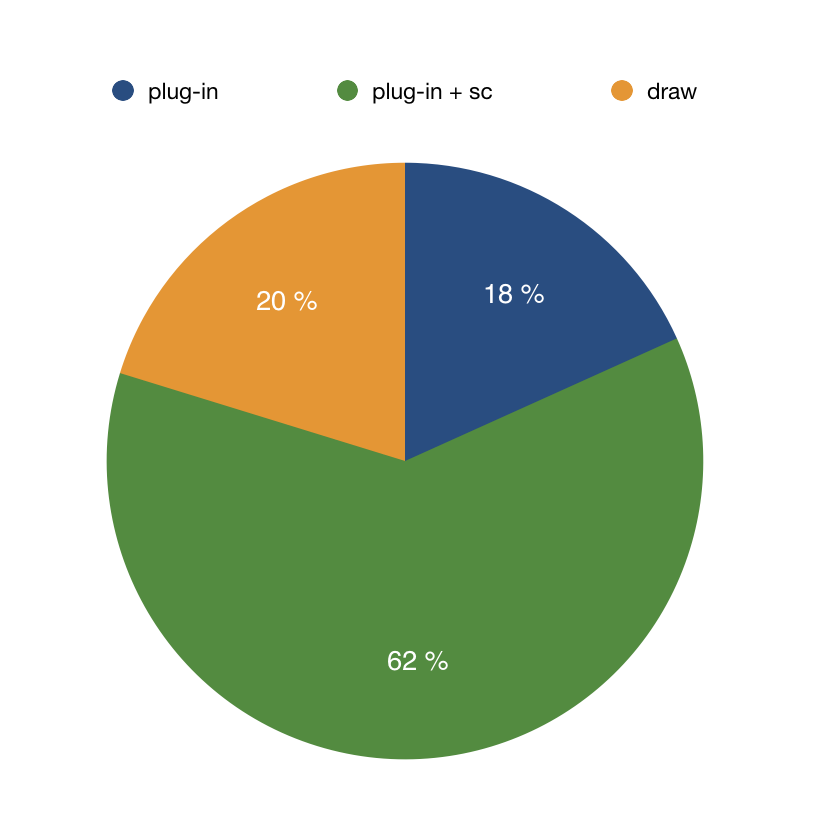
\includegraphics[width=0.55\textwidth]{images/betterRating}
	\centering
	\caption{Plug-in setting with better rating (all tests)}
	\label{b1}
\end{figure}
